\documentclass{article}
\usepackage{blindtext}
\usepackage[a4paper, total={6in, 9.4in}]{geometry}

\usepackage{wrapfig}
\usepackage{graphicx}
\usepackage{mathtext}
\usepackage{amsmath}
\usepackage{siunitx} % Required for alignment
\usepackage{subfigure}
\usepackage{multirow}
\usepackage{rotating}
\usepackage[T1,T2A]{fontenc}
\usepackage[russian]{babel}
\usepackage{caption}
\usepackage{physics}

\graphicspath{{pictures/}}

\title{\begin{center}Лабораторная работа №3.4.2\end{center}
Закон Кюри-Вейсса}
\author{Гёлецян А.Г.}
\date{\today}

\begin{document}

\pagenumbering{gobble}
\maketitle
\newpage
\pagenumbering{arabic}

\textbf{Цель работы:} изучение температурной зависимости магнитной восприимчивости ферромагнетика выше точки Кюри.

\textbf{В работе используются:} катушка самоиндукции с образцом из гадолиния, термостат, частометр, цифровой вольтметр, $ LC $-автогенератор, термопара медь-константин.

\section{Теоретическая часть}
\paragraph{Модель среднего поля.}
В качестве простейшей эмпирические модели, описывающей магнитную восприимчивость 
ферромагнетика, можно рассмотреть следующую модель: Пусть намагниченность среды 
пропорциональна некоторому эффективному полю $\vb* H_{эфф}$, складывающемуся из поля
$\vb* H$ в данной точке, созданного сторонними токами, и среднего "коллективного" 
поля, пропорционального величине намагниченности $\vb* M$
\begin{equation*}
    \vb* M = \chi_{пар}\vb* H_{эфф} \\
\end{equation*}
\begin{equation*}
    \chi_{пар} \propto 1/T \\
\end{equation*}
\begin{equation*}
    \vb* H_{эфф} = \vb* H + \beta \vb* M
\end{equation*}
Отсюда можно получить закон Кюри-Вейсса
\begin{equation}
    \label{Curie-Weiss}
    \chi = \frac{1}{\chi^{-1}_{пар} - \beta} \propto \frac{1}{T - \Theta}
\end{equation}

\section{Установка}

\begin{figure}[h]
    \center{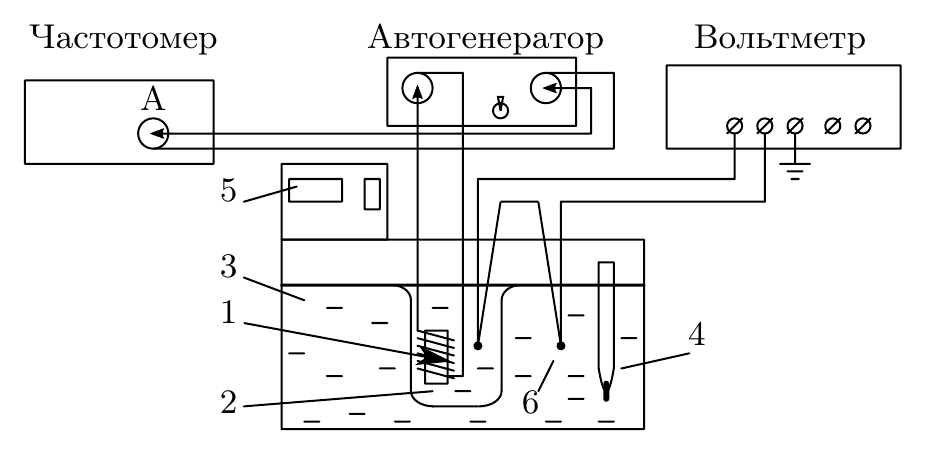
\includegraphics[scale=0.4]{ustanovka}}
    \caption{Установка для определения коэффициента вязкости жидкости.}
    \label{ustanovka}
    \newpage
\end{figure}


Установка измеряет температуру образца и собственный период колебания $LC$ контура, 
где $C$ находится в автогенераторе, а в качестве $L$ выступает катушка с гадолиниевым 
сердечником. Обозначим $L_0$ индуктивность катушки без сердечника. Тогда
\begin{equation*}
    L - L_0 \propto \mu - 1 = \chi
\end{equation*}
Так же мы знаем что
\begin{align*}
    \tau_0 &= 2\pi\sqrt{L_0C} \\
    \tau &= 2\pi\sqrt{LC} \\
\end{align*}
Подставляя уравнения и воспользовавшись законом Кюри-Вейсса (\ref{Curie-Weiss}) полуаем
\begin{equation}
    \frac{1}{\chi} \propto \frac{1}{\tau^2 - \tau_0^2} \propto T - \Theta_p
\end{equation}
Измерения температуры проводим двумя частями. Термометр измеряет температуру воды в 
термостате, а термопара измеряет разницу температур воды и масла в пробирке, в котором находится образец с катушкой. 

\section{Измерения}
Параметры установки
\begin{equation*}
    \tau_0 = (8.252 \pm 0.001) \mu с \mathrm{,}\quad \kappa = 24^\circ C/мВ
\end{equation*}
Температура масла в пробирке считается формулой
\begin{equation*}
    T = T_{вода} + \Delta T \quad \text{где} \quad \Delta T = \kappa U
\end{equation*}

\begin{table}[!h]
\begin{center}
\begin{tabular}{|l|r|r|r|}
\hline
 № & $T_{в}, ^\circ C$ & $U, мВ$ & $P, \mu с$\\ \hline
 1 & 11.09 &  -4 & 10.1612 \\
 2 & 13.07 &  -7 & 10.1070 \\
 3 & 14.05 &  -9 & 10.0683 \\
 4 & 16.06 &  -7 &  9.9403 \\\hline
 5 & 18.02 & -14 &  9.7542 \\
 6 & 20.02 & -14 &  9.4331 \\
 7 & 22.03 & -14 &  9.0214 \\
 8 & 24.01 & -17 &  8.7452 \\\hline
 9 & 26.02 & -18 &  8.6090 \\
10 & 28.01 & -20 &  8.5355 \\
11 & 30.01 & -20 &  8.4875 \\
12 & 32.00 & -20 &  8.4539 \\\hline
13 & 34.00 & -20 &  8.4290 \\
14 & 36.00 & -31 &  8.4126 \\
15 & 37.98 & -33 &  8.3984 \\
16 & 39.95 & -42 &  8.3874 \\\hline
\end{tabular}
\end{center}
\caption{Сырые данные}
\label{raw_data}
\end{table}

Ошибки сырых данных
\begin{equation*}
    \Delta T_{в} = 0.01 ^\circ C \mathrm{,}\quad
    \Delta U = 1мВ \mathrm{,}\quad\Delta
    P = 0.001 \mu c
\end{equation*}
После обработки данных получаем следующие значения, где $y=\frac{1}{\tau^2-\tau^2_0}$

\newpage

\begin{table}[!h]
\begin{center}
\begin{tabular}{|l|rr|rr|rr|}
\hline
№ & $T$ & $\Delta T,^\circ C$ & $\tau$ & $\Delta \tau, \mu с$ & $y$ & $\Delta y, \mu с^{-2}$\\\hline
 1 & 10.994 & 0.026 & 10.1612 & 0.001 & 0.028446 & 0.000021 \\
 2 & 12.902 & 0.026 & 10.1070 & 0.001 & 0.029363 & 0.000023 \\
 3 & 13.834 & 0.026 & 10.0683 & 0.001 & 0.030052 & 0.000024 \\
 4 & 15.892 & 0.026 &  9.9403 & 0.001 & 0.032558 & 0.000027 \\\hline
 5 & 17.684 & 0.026 &  9.7542 & 0.001 & 0.036970 & 0.000035 \\
 6 & 19.684 & 0.026 &  9.4331 & 0.001 & 0.047875 & 0.000057 \\
 7 & 21.694 & 0.026 &  9.0214 & 0.001 & 0.075244 & 0.00013  \\
 8 & 23.602 & 0.026 &  8.7452 & 0.001 & 0.119289 & 0.00034  \\\hline
 9 & 25.588 & 0.026 &  8.6090 & 0.001 & 0.166130 & 0.00065  \\
10 & 27.530 & 0.026 &  8.5355 & 0.001 & 0.210117 & 0.0010   \\
11 & 29.530 & 0.026 &  8.4875 & 0.001 & 0.253669 & 0.0015   \\
12 & 31.520 & 0.026 &  8.4539 & 0.001 & 0.296479 & 0.0020   \\\hline
13 & 33.520 & 0.026 &  8.4290 & 0.001 & 0.338692 & 0.0027   \\
14 & 35.256 & 0.026 &  8.4126 & 0.001 & 0.373645 & 0.0032   \\
15 & 37.188 & 0.026 &  8.3984 & 0.001 & 0.410236 & 0.0039   \\
16 & 38.942 & 0.026 &  8.3874 & 0.001 & 0.443858 & 0.0046   \\\hline
\end{tabular}
\end{center}
\caption{Данные после обработки}
\label{data}
\end{table}
Построим график $y=y(T)$

\begin{figure}[h]
    \center{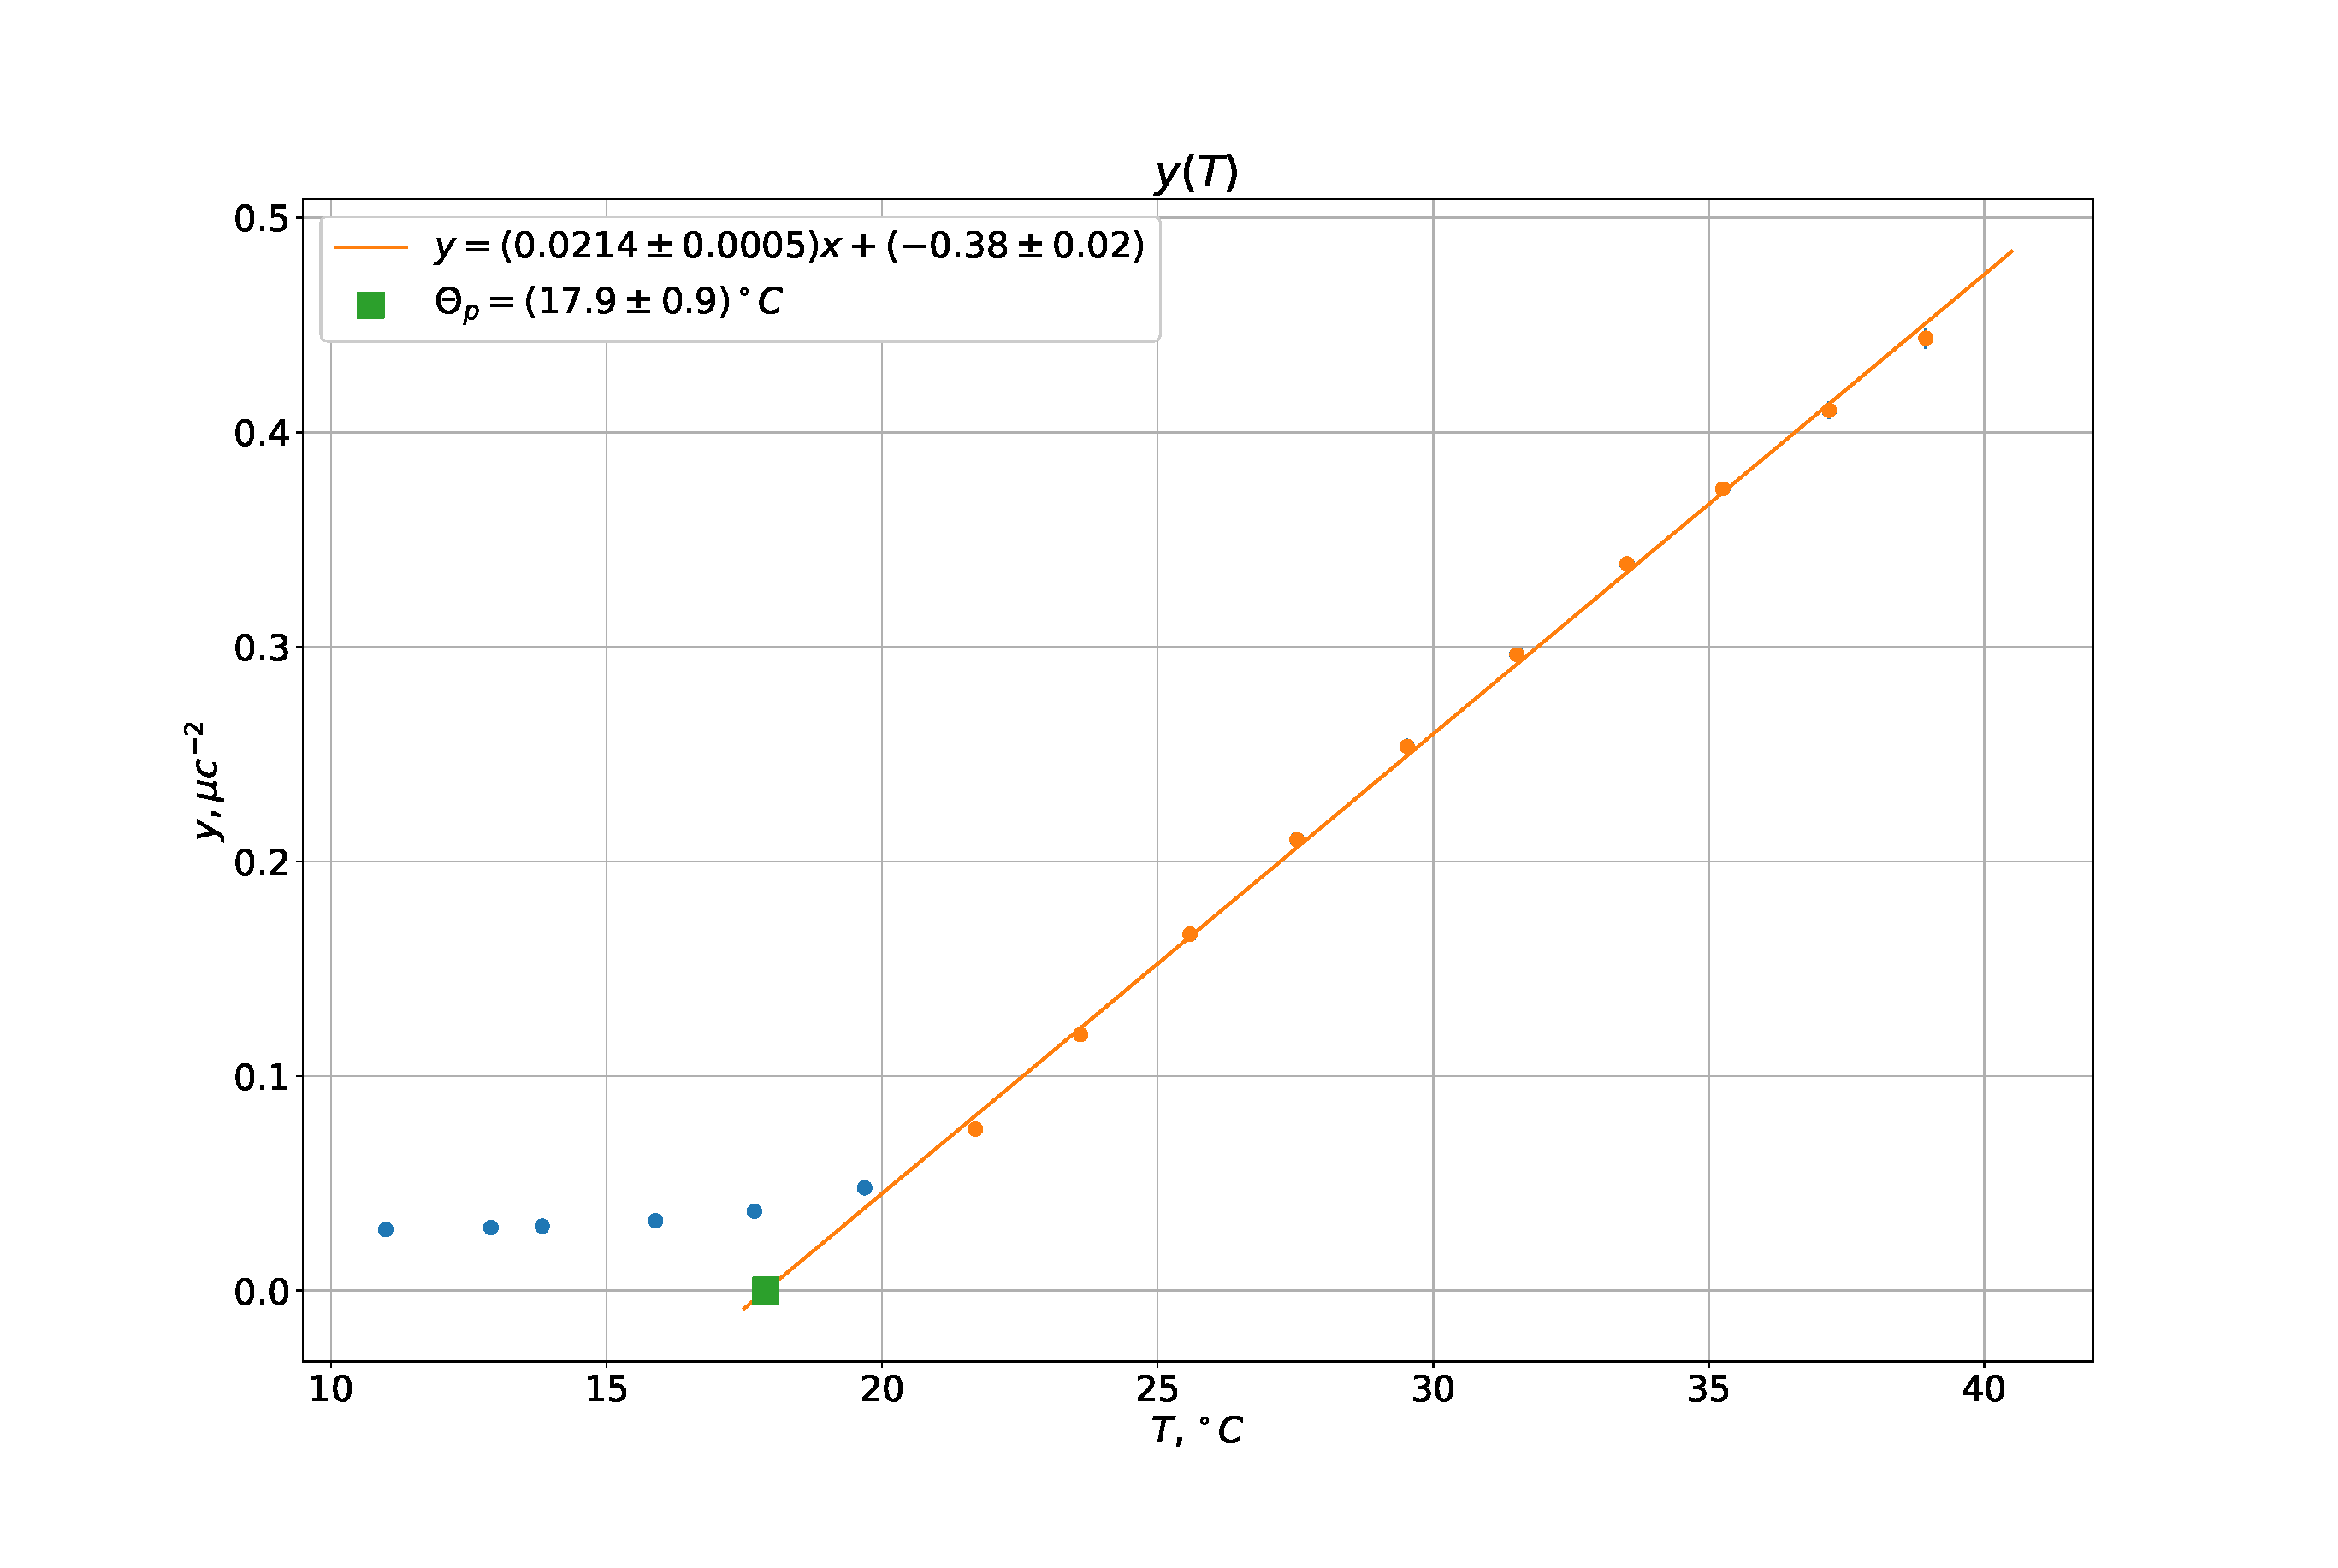
\includegraphics[width=0.85\textwidth]{plot}}
    \caption{График зависимости $y=y(T)$}
    \label{plot}
\end{figure}

Из графика получаем парамагнитную точку Кюри гадолиния
$\Theta_p = (17.9 \pm 0.9) ^\circ C$. Так же из графика можем оценить ферромагнитную 
точку Кюри $\Theta_{К} = (19.7 \pm 1) ^\circ C$

\newpage
\section{Выводы}
Из опыта получили следующие данные
\begin{equation}
    \Theta_p = (17.9 \pm 0.9) ^\circ C \mathrm{,}\quad \Theta_{К} = (19.7 \pm 1) ^\circ C
\end{equation}
Табличные значения этих данных
\begin{equation}
    \Theta_p^{таб} = (17.1 \pm 0.5) ^\circ C \mathrm{,}\quad
    \Theta_{К}^{таб} = 20.2 ^\circ C
\end{equation}
В пределах погрешности результаты совпадают с табличными значениями.

\end{document}

